\documentclass[12pt,letter]{article}
\usepackage{mathptmx} % added for time new roman font
\usepackage[left=1in,right=1in,top=1in,bottom=1in]{geometry}
\usepackage[latin1]{inputenc}
\usepackage{amsmath}

% defines all example enviorment
\usepackage[framemethod=tikz]{mdframed} % added for the box around examples
\newtheorem{ex}{Example}
\numberwithin{ex}{section} % allows for the use of example numbers that lign up with the section numbers
\newenvironment{example}{\begin{mdframed}[middlelinewidth=0.5mm]\begin{ex}\normalfont}{\end{ex}\end{mdframed}}

% defines all review enviorment
\usepackage[framemethod=tikz]{mdframed} % added for the box around examples
\newtheorem{re}{Review}
\numberwithin{re}{section} % allows for the use of example numbers that lign up with the section numbers
\newenvironment{review}{\begin{mdframed}[middlelinewidth=2mm,roundcorner=20pt]\begin{re}\normalfont}{\end{re}\end{mdframed}}

% defines the quotation enviorment 
\usepackage{xcolor}
\newcommand{\quotebox}[2]{\begin{center}\fcolorbox{white}{blue!15!gray!15}{\begin{minipage}{0.9\linewidth}\vspace{10pt}\center\begin{minipage}{0.8\linewidth}{\space\Huge``}{#1}{\Huge''}{\break\null\hfill} {\small #2}  \end{minipage}\medbreak\end{minipage}}\end{center}}

% defines the definition enviorment 
\newcommand{\definitionbox}[2]{\begin{center}\fcolorbox{white}{blue!15!gray!15}{\begin{minipage}{0.9\linewidth}\vspace{10pt}\center\begin{minipage}{0.8\linewidth} {{\textbf{Definition} - }{#1}: {#2}}\end{minipage}\medbreak\end{minipage}}\end{center}}

\usepackage{amsfonts}
\usepackage{amssymb}
\usepackage{graphicx}
\usepackage{float}
\usepackage{booktabs}
%\usepackage{parskip} % remove all the paragraph indents

\usepackage{setspace}
%\usepackage[colorlinks=true]{hyperref}
\usepackage{textcomp} 
\usepackage{multicol} 


%%%%%%%		define the symbols for positive directions		%%%%%%
\makeatletter													%%	
																%%					
\newcommand*\curveplus{% positive counterclockwise				%%
  \mathbin{\rotatebox[origin=c]{90}{$\m@th\curvearrowleft$}+}}	%%
																%%
\newcommand*\rightplus{% positive right							%%
  \mathpalette\@rightplus\relax}								%%
\newcommand*\@rightplus[1]{%									%%
  \mathbin{\vcenter{\hbox{$\m@th\overset{#1+}{\to}$}}}}			%%
																%%	
\newcommand*\upplus{% positive up								%%
  \mathbin{+\mathord\uparrow}}									%%
																%%			
\newcommand*\downplus{% positive down							%%		
  \mathbin{+\mathord\downarrow}}								%%
  																%%		
\newcommand*\downrightplus{% positive down and right			%%	
  \mathbin{+ \rotatebox[origin=c]{-30}{$\m@th\rightarrow$}}}	%%
\makeatother 													%%	
%%%%%%%%%%%%%%%%%%%%%%%%%%%%%%%%%%%%%%%%%%%%%%%%%%%%%%%%%%%%%%%%%%


\usepackage{mathtools}          %loads amsmath as well added for the piece wise function
\DeclarePairedDelimiter\Floor\lfloor\rfloor
\DeclarePairedDelimiter\Ceil\lceil\rceil

 
\newcounter{NumberInTable}
\newcommand{\LTNUM}{\stepcounter{NumberInTable}{(\theNumberInTable)}}

\newcommand{\Laplace}[1]{\ensuremath{\mathcal{L}{\left[#1\right]}}}
\newcommand{\InvLap}[1]{\ensuremath{\mathcal{L}^{-1}{\left[#1\right]}}}
\renewcommand{\textuparrow}{$\uparrow$}

\begin{document}
	
	\large{}
	
	\title{\vspace{-2cm} Chapter 1: Fundamentals of Vibrations}
	\date{}
	\maketitle

	\section{Basic Concepts in Vibrations}

    The study of vibrations, within the broader field of classical mechanics, is the investigation of oscillations that occur about an equilibrium point. Vibrations, both desired and undesired, are present in all mechanical systems and can be helpful (e.g. a soil sieve, rotary sander) or destructive (e.g. an aircraft frame in resonance). The oscillations that form a vibrating system may be periodic (e.g., pendulum) or random (e.g. turbulence in an airplane), or a combination of the two. 

    Vibrations impact our daily lives in a variety of ways, from the sound made by banjo strings that vibrates between 140 and 400 Hz to the 4-6 Hz vibration felt by a passenger in a car seat. The consideration of the vibrations and their associated mathematical modeling are an important factor in the design of mechanical systems. In the material that follows, the fundamental theories of vibration are presented and modeled using fundamental physical principles such and Newton's three laws of motion. These models and analyzed using the mathematical tools of calculus and differential equations. 

	\begin{review}
		Newton's three laws of motion:
		\begin{enumerate}
			\item In an inertial frame of reference, an object either remains at rest or continues to move at a constant velocity, unless acted upon by a force.
			\item In an inertial reference frame, the vector sum of the forces $F$ on an object is equal to the mass m of that object multiplied by the acceleration of the object: $F = ma$. (It is assumed here that the mass m is constant)
			\item When one body exerts a force on a second body, the second body simultaneously exerts a force equal in magnitude and opposite in direction on the first body.
		\end{enumerate}
	\end{review}

	\subsection{Single Degree-of-Freedom Systems}
	
        In its simplest form, the phenomenon of vibration is the exchange of energy between potential and kinetic energy. Therefore, a vibrating system must have a component that stores potential energy. This component must also be capable of releasing the energy as kinetic energy. This kinetic energy is stored in the movement of a mass where the measure of this movement is the velocity of the system and the continuous interchange between potential and kinetic energy is the vibration of the system. The simplest vibrating systems can be modeled as a single-degree-of-freedom (1-DOF) system. In a 1-DOF system, one variable can describe the motion of a system. Potential examples of  1-DOF systems include:
		
		\begin{enumerate}
			\item yo-yo
			\item pogo stick
			\item door swinging on axis
			\item throttle (gas pedal)
		\end{enumerate}
				
		\noindent Variables often used for describing 1-DOF systems are $x(t)$,  $y(t)$,  $z(t)$, and  $\theta(t)$.  Examples of 1-DOF systems are presented in figure \ref{fig:Examples_of_1DOF_systems} where the assumption of small displacements is made. Note: we will often drop the ``$(t)$'' for simplicity in this material. 

		\begin{figure}[H]
			\centering
			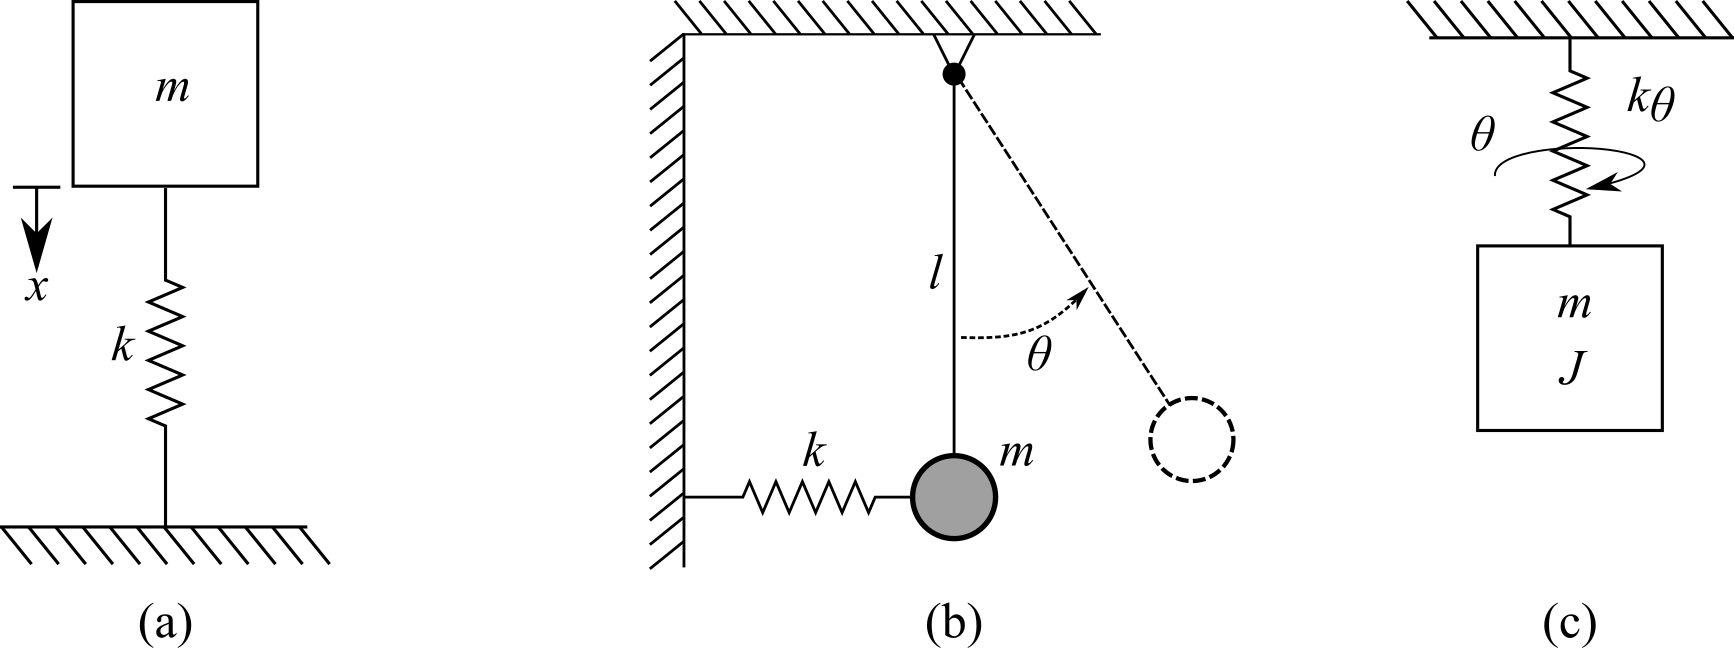
\includegraphics[]{../figures/Examples_of_1DOF_systems.png}
			\caption{Examples of single degree of freedom (DOF) systems showing: (a) a vertical spring-mass system; (b) a simple pendulum; and (c) a rotational spring-mass system.}
			\label{fig:Examples_of_1DOF_systems}
		\end{figure}

		\subsubsection{Spring-Mass Model}

			\quotebox{All models are wrong, but some are useful}{George E.P. Box (1919 - 2013)}	
							
            Newtonian physics describes the motion of particles in terms of displacement $x$, velocity $\dot{x}$, and acceleration $\ddot{x}$ vectors. Moreover, from Newton's second law of motion says that the change in the velocity of mass in motion is a product of the force acting on the mass. A simple way to express this phenomenon is though a spring-mass model as presented in figure  \ref{fig:spring_mass_model_with_point_mass}. These spring-mass models neglect the mass of the spring and concentrate all the mass of the system into a single point. Note that in this case the force vector and mass-acceleration vectors lie on the same axis and as such are collinear. Therefore, these vectors can be easily treated as scalers simplifying the math used in the modeling of the system.     

			\begin{figure}[H]
				\centering
				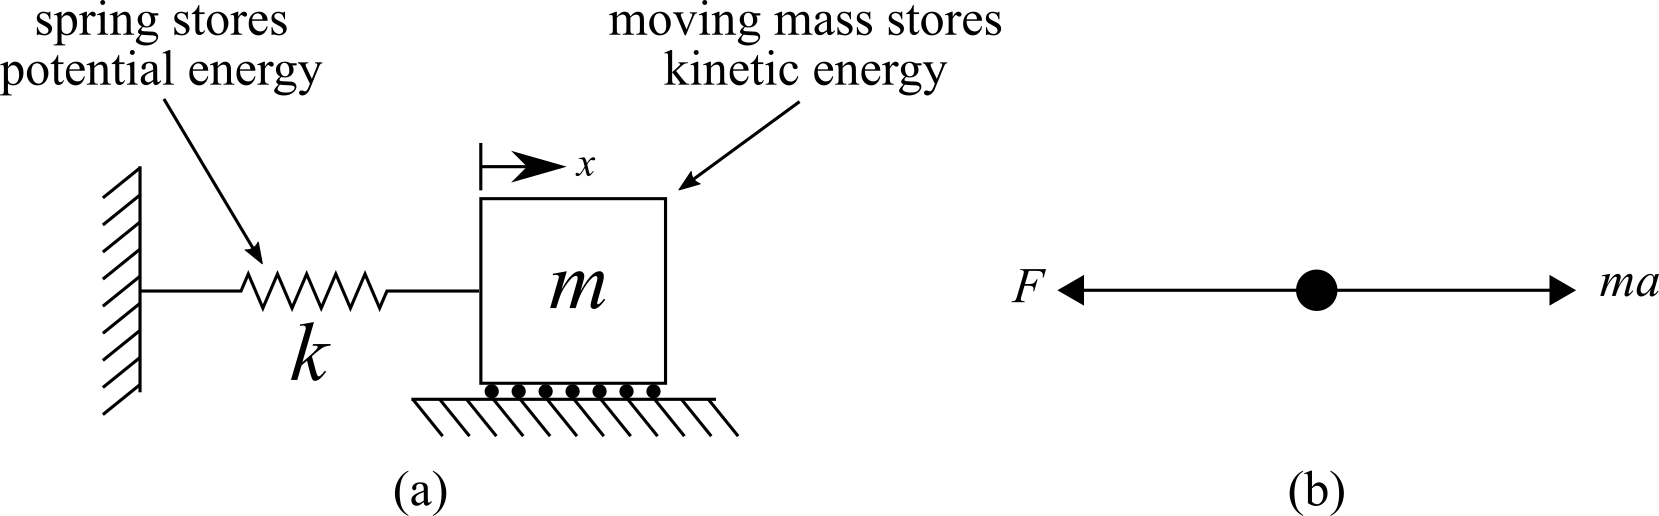
\includegraphics[]{../figures/spring_mass_model_with_point_mass.png}
				\caption{A single-degree-of-freedom (1-DOF) spring mass model showing: (a) annotated schematic of a mass-spring system; and (b) the equivalent free-body diagram represented as a point-mass system.}
				\label{fig:spring_mass_model_with_point_mass}
			\end{figure}	
		
		\subsubsection{Linear Springs}
	
            Springs are mechanical devices that store energy, moreover, ideal spring is a theoretical representation of this mechanical device that is massless and responds with a linear increase in force for a unit increase in displacement (i.e. $F=kx$). For simplicity, the spring in the spring-mass model considered here is assumed aways ideal linear springs. A graphical representation of the idealized linear spring is presented in figure \ref{fig:linear_spring_deformation} where a unit force $F$ applied to the free end of the spring results in a unite displacement $x$ of the spring.  The resulting mathematical relationships,  $F=kx$, is known as Hooke's Law. Nonlinear springs add considerable complexity to the modeling of spring-mass systems, therefore, these are not considered in this introductory work. 
			
			\begin{figure}[H]
				\centering
				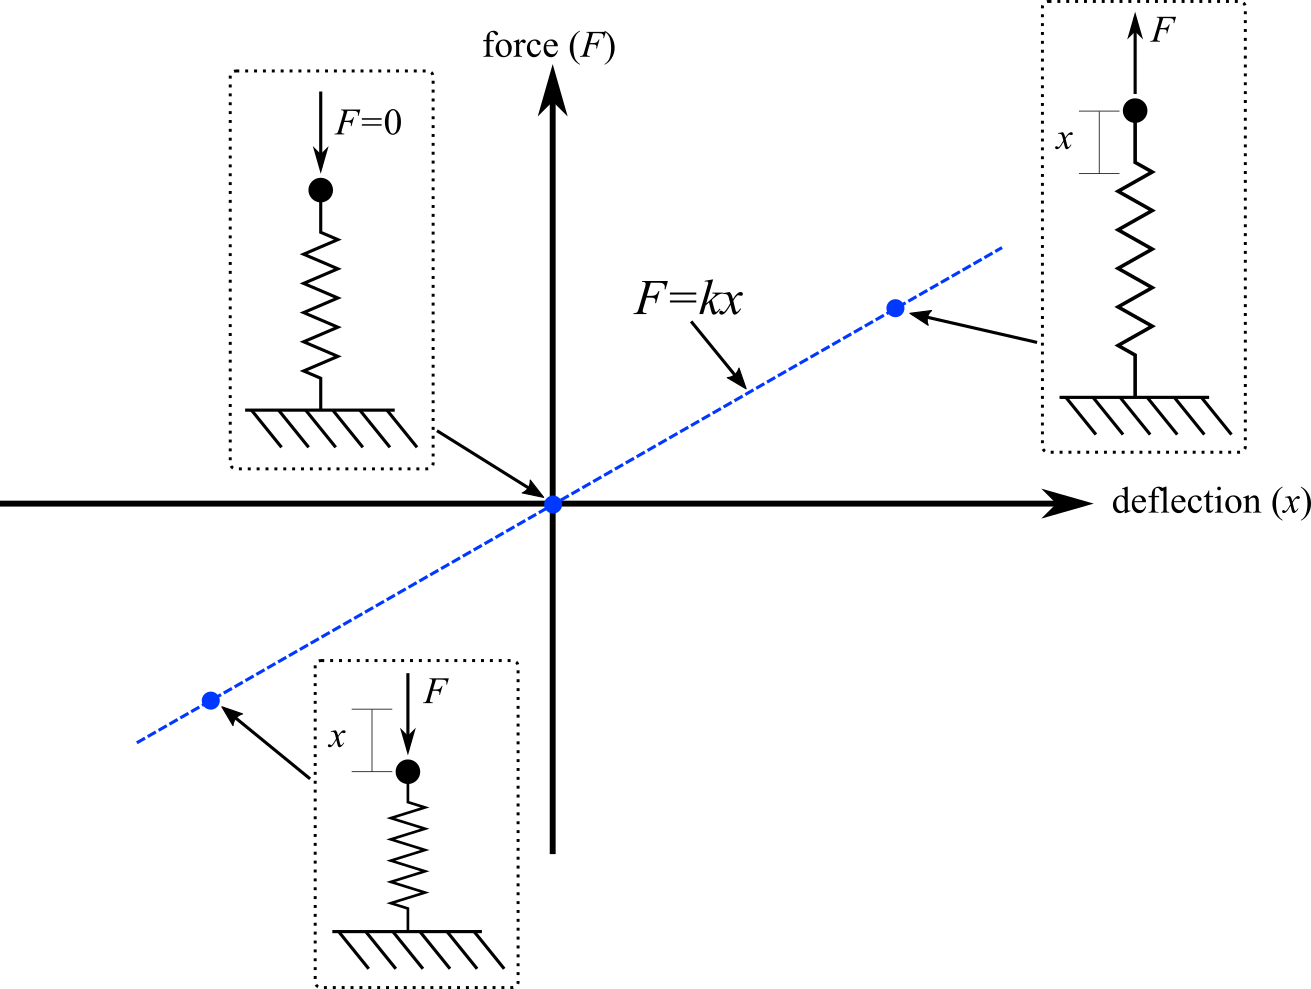
\includegraphics[]{../figures/linear_spring_deformation.png}
				\caption{Force-displacement plot for a linear spring.}
				\label{fig:linear_spring_deformation}
			\end{figure}					


	\subsection{Equivalent Stiffness}
		
		The generalized concept of stiffness can be directly related to mechanical systems and structural components through Hooke's law. 	\begin{review}
			Hooke's Law states that the force ($F$) needed to extend or compress a spring by some distance $x$ scales linearly with respect to that distance. This law can be extend to tensional stress of an uniform and elastic bar where the length, area, and Young's modulus of the bar are represented by $l$, $A$, and $E$, respectively. Knowing the tensile stress in the bar:
			\begin{equation}
			\sigma = \frac{F}{A}
			\end{equation} 			
			and the definition of strain:
			\begin{equation}
			\varepsilon = \frac{\Delta l}{l}
			\end{equation} 			
			Hooke's law can be expanded to represent an uniform and elastic bar:
			\begin{equation}
			\sigma = E \varepsilon
			\end{equation} 			
			It follows that the change in length $\Delta l$ can be expressed as:		
			\begin{equation}
			\Delta l = \varepsilon l = \frac{F L}{A E}
			\end{equation} 
			\textbf{Note:} Hooke's law is often expressed using the convention that $F$ is the restoring force exerted by the spring on the applied force at the free end. Using this expression, the equation for Hooke's Law becomes:
			\begin{equation}
			F = -kx
			\end{equation} 			
			since the direction of the restoring force is opposite the spring displacement.
		\end{review}
	
		\subsubsection{Equivalent Stiffness of Structural Systems}	
		
            For a rod with a uniform cross-section, a direct representation of the system can be developed as expressed in figure \ref{fig:spring_and_bar_mass_vertical} where the vibration along the axis of the rod is to be considered. The stiffness of the rod, $k$, is a measure of the resistance offered by an elastic body to deformation. 

			
			\begin{figure}[H]
				\centering
				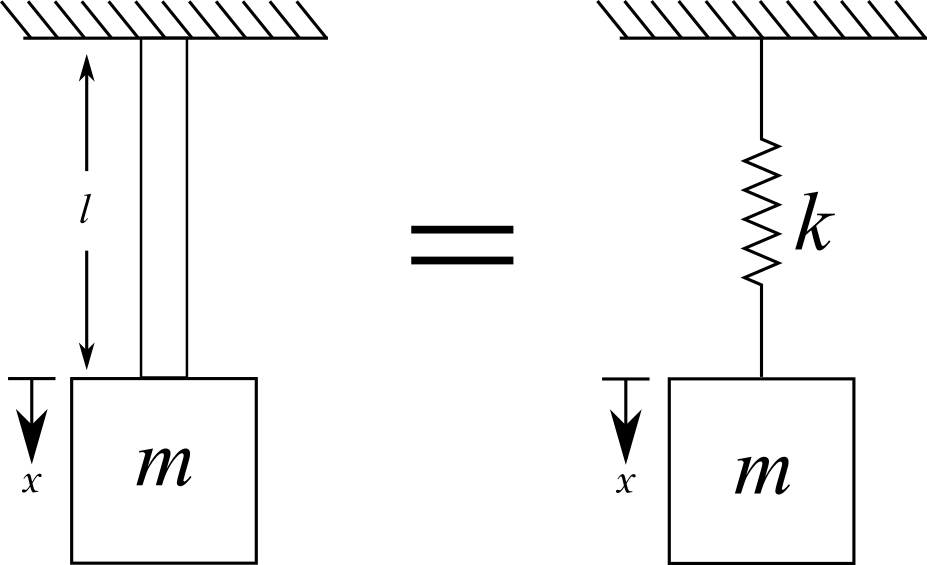
\includegraphics[]{../figures/spring_and_bar_mass_vertical.png}
				\caption{Equivalency between a vertical bar with mass attached to the bottom and a spring-mass model of the system}.
				\label{fig:spring_and_bar_mass_vertical}
			\end{figure}
			
			For this 1-DOF system, the equation of a spring can be rearranged such that the stiffness can be defined as:
			\begin{equation}
				k=\frac{F}{x}
			\end{equation}
			The stiffness of the spring can be more closely related to materials properties of the bar $A$, $E$, and $l$ considering that Hooke's Law for the uniform tension on a bar can be expressed as:
			\begin{equation}
				\sigma = E \varepsilon
			\end{equation}			
			This expression can be expanded into the form:
			\begin{equation}
				\frac{F}{A} = E \Big( \frac{x}{l} \Big)
			\end{equation}					
			rearranging the terms and recalling the expression $k = \frac{F}{x}$ leads to:			
			\begin{equation}
				 k = \frac{EA}{l}
			\end{equation}				
		
			In a similar fashion, we can also solve the equivalent system for a mass at the end of a cantilever beam.
			\begin{figure}[H]
				\centering
				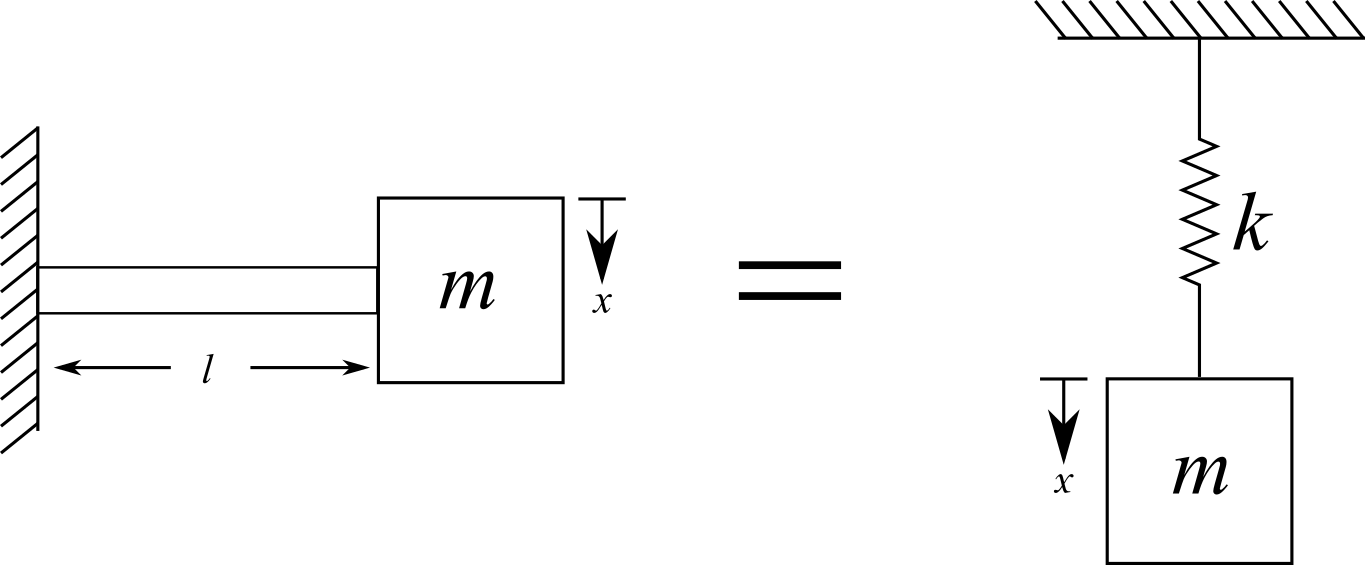
\includegraphics[]{../figures/spring_and_bar_mass_cantilever_beam.png}
			\end{figure}			
			From engineering mechanics we can compute the deflection at the point of a beam $\delta$ with a point load $P$. This expression is typically expressed as:
			\begin{equation}
				\delta = \frac{Pl^3}{3EI}
			\end{equation}					
			If we transform this matrix into our variable system by exchanging $P$ for $F$ and $\delta$ for $x$. Thereafter, the point load is replaced with the equivalent force $F$ generated by the mass and the pull of gravity($mg$). As before, knowing that the stiffness of the system can be expressed as $x=F/x$ we can show that:
			\begin{equation}
				k = \frac{3EI}{l^3}
			\end{equation}	


			\begin{example}
    			
    			Considering the rod diagrammed below; calculate an equivalent spring constant for the rod using the length of the rod $l$, its area $A$, and Young's modulus $E$ for a compressive force $F$ that compresses the rod a distance $x$. Additionally, is a linear spring a useful model for a rod under compression? What if the rod is under tension?
        
		 		\begin{figure}[H]
		 			\centering
		 			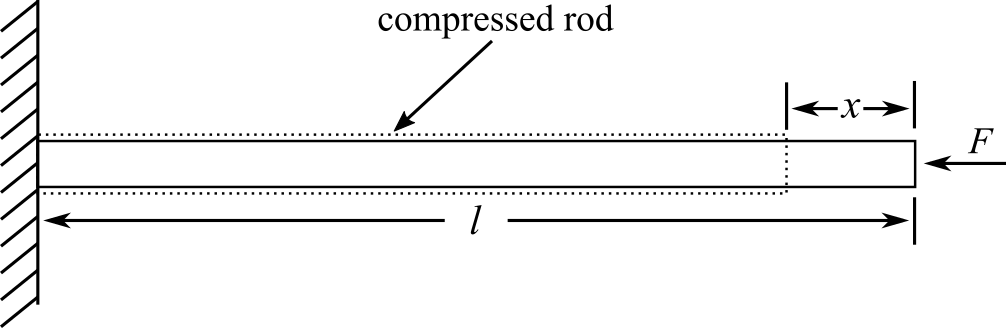
\includegraphics[]{../figures/compressed_cantilever_rod.png}
		 			\caption{Compressed cantilever rod. }
		 		\end{figure}	   
       
			    \textbf{Solution:} The rod shortens by a distance $x$ under the axial force $F$, this can be related to the equation of a linear spring $F=kx$ by recalling from solid mechanics that the elongation (or shortening) of a rod is expressed as 
			
			    \begin{eqnarray}
			    x=\frac{x}{l}l=\varepsilon l = \frac{\sigma}{E}l = \frac{Fl}{AE}
			    \end{eqnarray}    
			    
			    where  $\varepsilon = \frac{x}{l}$ is the strain value and $\sigma = F/A$ is the stress induced in the rod. Combining this expression with the equation of a linear spring yields:
			    
			    \begin{eqnarray}
			    k = \frac{F}{x}= \frac{AE}{l}
			    \end{eqnarray}     
			   
			    As per the usefulness of the linear spring to represent an axial rod under compression or tension, this would be application-specific but could generally be considered an excellent first-order approximation.  
			
			\end{example}

		\subsubsection{Springs in Series and Parallel}
			
			In many cases, it becomes necessary to model a mechanical system as a set of springs (e.g., a composite material, a table with multiple legs).  For these systems, or for systems with more than one spring acting on a body, equivalent stiffness can be calculated as:
			\begin{figure}[H]
				\centering
				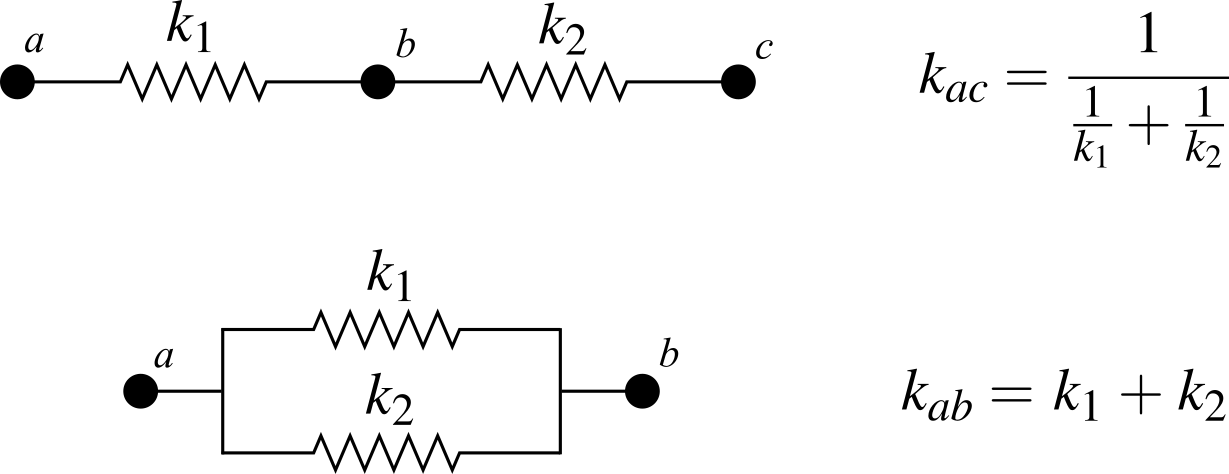
\includegraphics[]{../figures/equivalent_stiffness.png}
				\caption{Equations for calculating the equivalent stiffness of two springs ($k_1$ and $k_2$); (a) in series; and (b) in parallel.}
			\end{figure}	
			These are derived considering the displacement $\delta$ of the systems. For two springs in series:
			\begin{figure}[H]
				\centering
				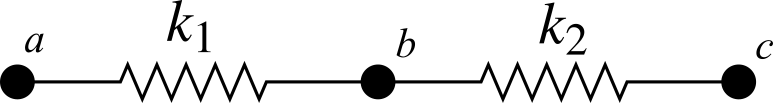
\includegraphics[]{../figures/equivalent_stiffness_series.png}
				\caption{Two springs $k_1$ and $k_2$ combined in series.}
			\end{figure}			
			\noindent where the total displacement is 
			\begin{equation}
				\delta_{ac} = \delta_{ab} + \delta_{bc}
			\end{equation}
			Using the equation for stiffness $k=F/\delta$, this converts to:
			\begin{equation}
				\frac{F}{k_{ac}} = \frac{F}{k_{1}} + \frac{F}{k_{2}}
			\end{equation}
			As $F$ is the same throughout the system, we can cancel out $F$. Solving for the equivalent stiffness yields:
			\begin{equation}
				k_{ac} = \frac{1}{\frac{1}{k_1}+\frac{1}{k_2}}
			\end{equation}
			Similarly for a system of springs in parallel:
			\begin{figure}[H]
				\centering
				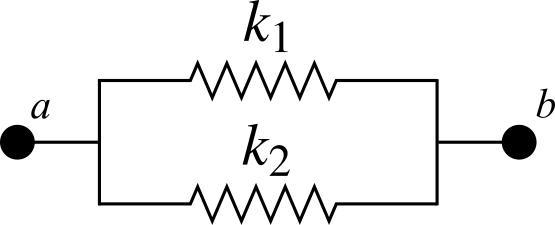
\includegraphics[]{../figures/equivalent_stiffness_parallel.png}
				\caption{Two springs $k_1$ and $k_2$ combined in parallel.}				
			\end{figure}			
			\noindent The displacement in both springs is the same, so the total displacement is 
			\begin{equation}
				\delta_{ab} = \delta_{\text{1}} =  \delta_{\text{2}} = \delta
			\end{equation}
			The forces in the direction of spring elongation sum to zero, therefore:
			\begin{equation}
				F_{ab} = F_{\text{1}} +  F_{\text{2}}
			\end{equation}			
			Substituting the displacement and stiffness into the force equation yields:
			\begin{equation}
				\delta k_{ab} = 	\delta k_{1} +  \delta k_{2}
			\end{equation}				
			this simplifies to:
			\begin{equation}
				k_{ab} = k_1+k_2
			\end{equation}
			


			\begin{example}

				Calculate the equivalent stiffness of the following system:
				\begin{figure}[H]
					\centering
					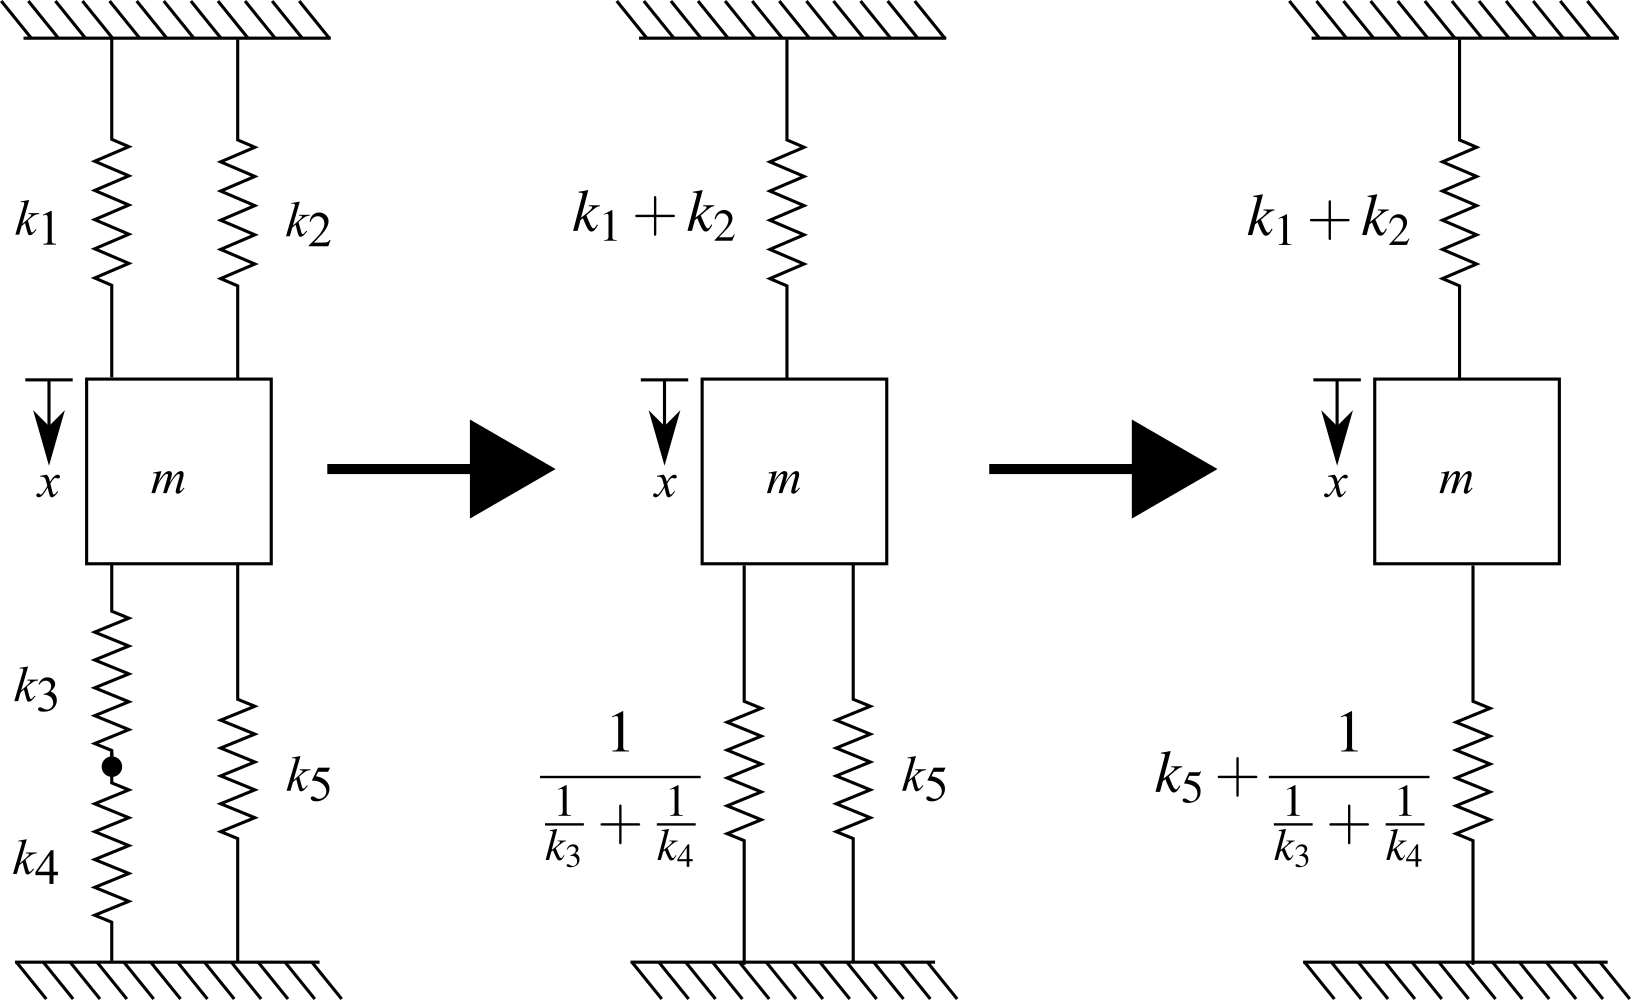
\includegraphics[]{../figures/equivalent_mass_and_spring_system_1.png}
				\end{figure}	
				The springs are combined as shown, using the equations defined before.  Now, considering that the displacement ($\delta$) of the top spring, and the bottom spring are the same we can state the total stiffness $k$, is the summation of the two. Therefore,    
				\begin{figure}[H]
					\centering
					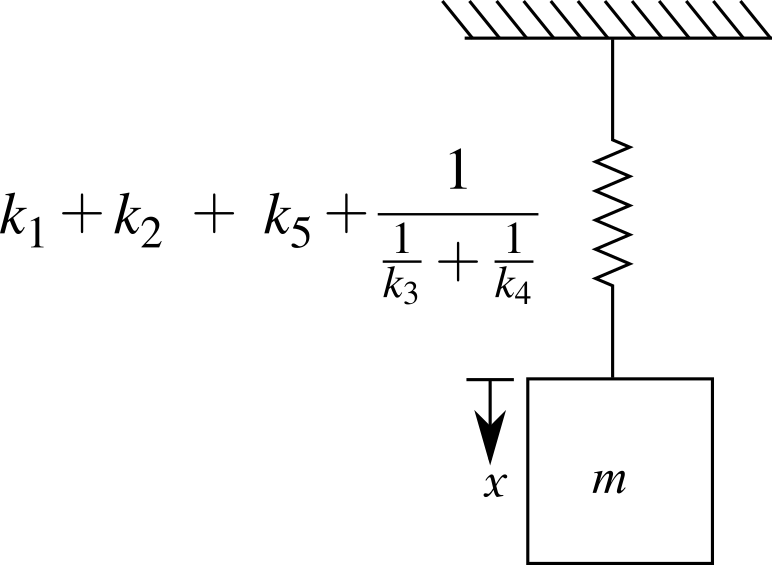
\includegraphics[]{../figures/equivalent_mass_and_spring_system_2.png}
				\end{figure}	
%				until a final $k$ value can be obtained:
%				\begin{equation}
%					k=k_1+k_2+k_5+\frac{1}{\frac{1}{k_3}+\frac{1}{k_4}}
%				\end{equation}		
				\noindent where the final addition, $(k_1+k_2) + (k_5+\frac{1}{\frac{1}{k_3}+\frac{1}{k_4}})$ is applied at two springs in parallel as each spring is connected between the mass and the fixity. Rearranging this new expression to get a common denominator:
				\begin{equation}
					k= \frac{(k_1+k_2+k_5)(k_3+k_4)+k_3k_4}{k_3+k_4}  
				\end{equation}				
%				For an arbitrary mass, $m$, the undamped frequency $\omega_n$ can be calculated as:
%				\begin{equation}
%					\omega_n = \sqrt{\frac{k}{m}} = \sqrt{\frac{(k_1+k_2+k_5)(k_3+k_4)+k_3k_4}{m(k_3+k_4)} }
%				\end{equation}				
			\end{example}	

					
	\subsection{Equation of Motion for an Oscillating System}			
			
        An Equation of Motion (EOM) is an equation that provides a basis for modeling a vibrating system about its equilibrium point and relates the transfer of the potential energy from the spring to the kinetic energy mass. In developing the EOM we assume that any surfaces are frictionless and as such, no energy is extracted from the vibrating system. Referencing the 1-DOF system in figure \ref{fig:EOM_1-DOF-mass_horizontal}(a), and assuming the mass only moves in the $x$ direction, the only force acting on the mass in the $x$ direction is the force that results from the elongation of the spring as annotated in figure \ref{fig:EOM_1-DOF-mass_horizontal}(b). Therefore, the sum of forces in along the $x$ axis must equal the mass ($m$) times the acceleration of the mass ($a\dot{x}$). 

		\begin{figure}[H]
			\centering
			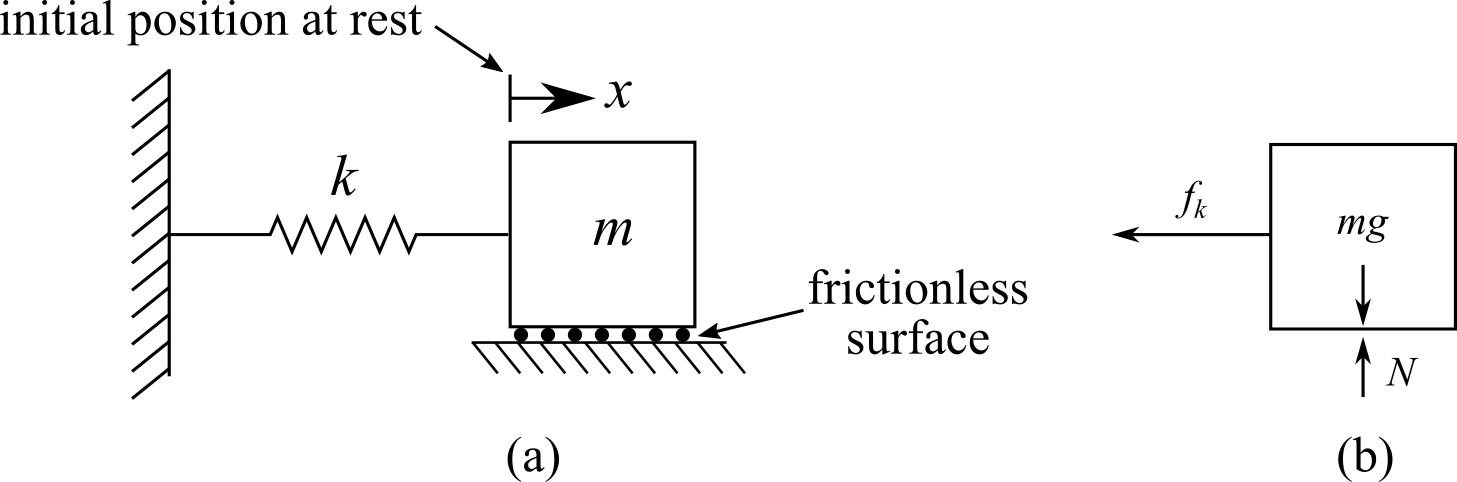
\includegraphics[]{../figures/EOM_1-DOF-mass_horizontal.png}
			\caption{A spring mass model of a 1-DOF system showing: (a) a schematic of the system; (b)  free-body diagram of the system at its initial position.}
			\label{fig:EOM_1-DOF-mass_horizontal}
		\end{figure}			
		
		Considering that positive displacements are to the right, the standard form of the equation of motion for an undamped system without any excitation is expressed as:  
		\begin{equation}
			s_1 \ddot{x} + s_2 x = 0
		\end{equation}			
		where $s_1$ and $s_2$ are constants to be determined for the specific system. A systematic approach to obtaining free-body diagram (FBD) of a system under vibration can be expressed in three steps:
		\begin{enumerate}
			\item Draw a free-body diagram (FBD) at the system's equilibrium and displaced position (without a displacing force).
			\item Apply Newton's second law to both FBDs ( equilibrium and displaced).
			\item Combine the equations to write the EOM in standard form with the forcing component on the right-hand side. For free vibration, the forcing component is 0. 
		\end{enumerate}
			
		Solving these three steps for 1-DOF system presented in figure \ref{fig:EOM_1-DOF-mass_horizontal} results in the EOM:
		\begin{equation}
			m \ddot{x} + k x = 0
		\end{equation}

		\begin{review}
			A second-order linear homogeneous differential equation has the form:
			
			\begin{equation}
			 a \ddot{x} + b \dot{x} + cx = 0
			\end{equation}
		
			\noindent The EOM for a 1-DOF system under a free vibration is a a second-order differential equation due to acceleration ($\ddot{x}$) being the second derivative of displacement ($x$) and homogeneous as the forcing function (right-hand side of the equations) is zero. In EOM's current form, $m=k$, $b=0$,  and $c=k$. In future work, $b$ will account for damping in the vibrating system.     
		\end{review}

					
		\begin{example}			
			
			Considering the system:
			\begin{figure}[H]
				\centering
				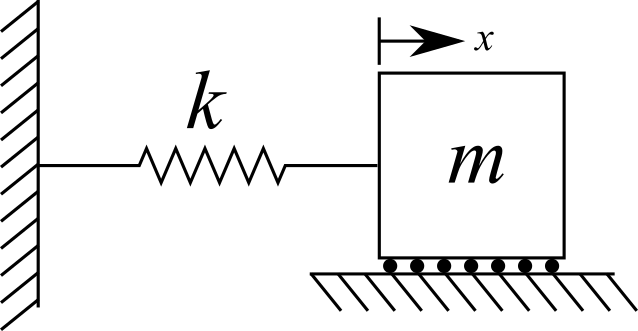
\includegraphics[]{../figures/1-DOF-mass_horizontal.png}
			\end{figure}		
			
			\textbf{Step-1}
			Define the direction of displacement, and draw the FBD for the equilibrium and displaced state.  
			\begin{figure}[H]
				\centering
				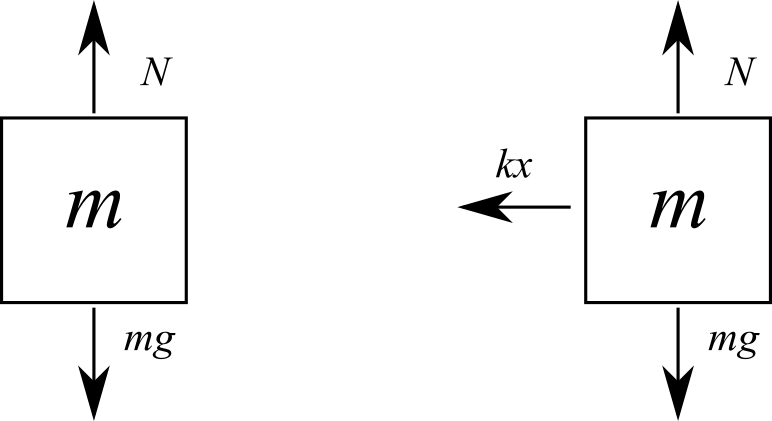
\includegraphics[width=0.45\textwidth]{../figures/1-DOF-mass_horizontal_FBD.png}\\
				equilibrium state \hspace{3cm} displaced state
			\end{figure}		
			\noindent The equation for the equilibrium state is:
			\begin{equation}
			\rightplus \sum F_x = 0
			\end{equation}
			and in the displaced state:
			\begin{equation}
			\rightplus \sum F_x = -kx
			\end{equation}		
			This equation does not equal zero as the FBD does not account for the restoring force. 
	
			\noindent	\textbf{Step-2} Apply Newton's second law (we want to store energy in the kinetic state) of motion to the sum of forces for the displaced position we get: 		 		
			\begin{equation}
			ma = m\ddot{x} = \rightplus \sum F_x = -kx
			\end{equation}			
			\begin{equation}
			m\ddot{x} = -kx
			\end{equation}				
			\textbf{Step-3} Rearrange in the Equation to construct an EOM: 			
			\begin{equation}
			m\ddot{x} + kx = 0
			\end{equation}		
		\end{example}			

		\begin{example}	
			Some systems will have an initial displacement, as the system will oscillate around this position we need to define the EOM about this position. Considering the system:
			\begin{figure}[H]
				\centering
				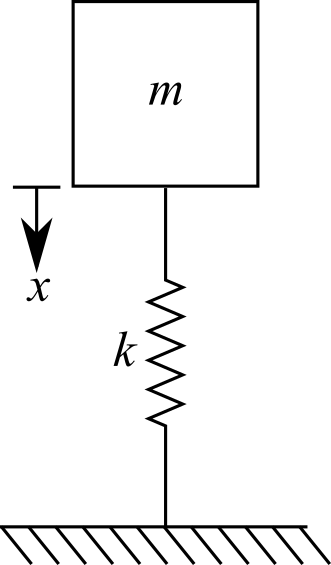
\includegraphics[]{../figures/1-DOF-mass_vertical.png}
			\end{figure}		
			\noindent \textbf{Step-1}
			Define the direction of displacement, and draw the FBD for the equilibrium and displaced state.  
			\begin{figure}[H]
				\centering
				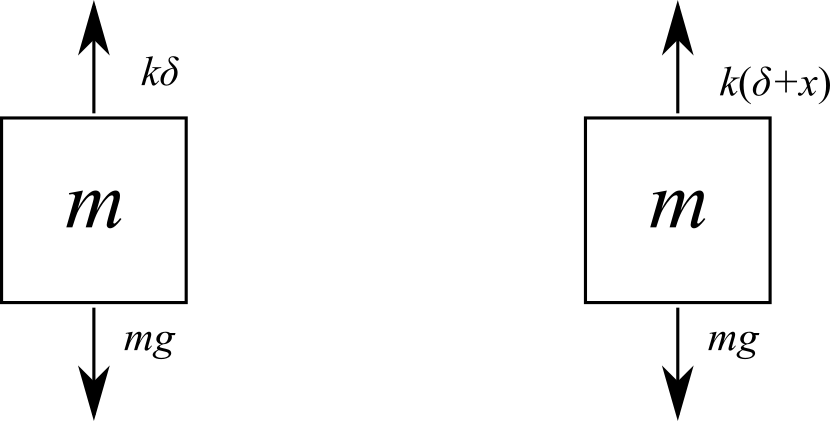
\includegraphics[]{../figures/1-DOF-mass_vertical_FBD.png}\\
				equilibrium state \hspace{3cm} displaced state
			\end{figure}		
			\noindent The equation for the equilibrium state is:
			\begin{equation}
				\downplus \sum F_x = mg - k\delta = 0
			\end{equation}
			and in the displaced state:
			\begin{equation}
				\downplus \sum F_x =mg -k(\delta + x)
			\end{equation}	
			This equation does not equal zero as the FBD does not account for the restoring force.	
			
			\noindent \textbf{Step-2} Apply Newton's second law (we want to store energy in the kinetic state) of motion to the sum of forces for the displaced position we get: 		
			\begin{equation}
				m\ddot{x} = \downplus \sum F_x =mg -k\delta -kx
			\end{equation}
			We can than use the information from the equilibrium state to cancel out some terms, this becomes:
			\begin{equation}
				m\ddot{x} = -kx
			\end{equation}				
			\textbf{Step-3} Rearrange in the Equation to construct an EOM: 					
			\begin{equation}
				m\ddot{x} + kx = 0
			\end{equation}			
		\end{example}		
		
\end{document}

